%+ ======================================================================================================================
%+ Noi dung: PHU LUC
%+ ======================================================================================================================
\chapter*{Phụ lục}
Phụ lục này sẽ trình bày một số modules cơ bản của thuật toán đơn hình gốc của Dantzig ,và một số module của phương pháp phân rã Dantzig-Wolfe dưới dạng ngôn ngữ Visual Basic, phiên bản 6.0.

Cụ thể sẽ trình bày các thủ tục sau:\\
\noindent{\bf 1. Modul thuật toán đơn hình gốc của Dantzig}
{\footnotesize
\\noindent{\bf 1. Modul thuật toán đơn hình gốc của Dantzig}
\begin{verbatim}
Private Sub QHTT()
    'Bo xung vao ma tran A
    Dim i, j As Integer
    Dim b_temp(30) As Double
    Dim a_temp(100, 100) As Double
    For i = 0 To m - 1
        a(i + 1, 0) = b(i + 1) 'Cot 0 ma tran a
    Next
    For i = 0 To n - 1
        a(0, i + 1) = c(i + 1)
    Next
    
    'Phuong phap don hinh
    Dim toi_uu As Boolean
    toi_uu = False
    Dim var_lap As Integer
    var_lap = 0
    While toi_uu = False
        'Tinh cac uoc luong delta
        For j = 1 To n
            a(m + 1, j) = 0
            For i = 1 To m
                a(m + 1, j) = a(m + 1, j) + acb(i) * a(i, j)
            Next
            a(m + 1, j) = a(m + 1, j) - a(0, j) 
			'Dong thu m+1 trong ma tran a luu tru cac gia tri delta
        Next
        
        ' Hien thi bang don hinh
        display (var_lap * (m + 2) + 1)
        
        'Tim delta max va s
        Dim s As Integer
        s = 1
        Dim delta As Double
        delta = a(m + 1, s)
        For j = 1 To n
            If a(m + 1, j) > delta Then
                delta = a(m + 1, j)
                s = j
            End If
        Next
        'MsgBox (CStr(delta))
        
        ' Kiem tra dieu kien toi uu
        If delta > 0 Then
            toi_uu = False
        Else
            toi_uu = True
            GoTo Ketthuc
        End If
        
        'Kiem tra vo nghiem
        Dim voNo As Boolean
        voNo = False
        For j = 1 To n
            If a(m + 1, j) > 0 Then
                dem = 1
                Do While dem <= m And a(dem, j) <= 0
                    dem = dem + 1
                Loop
                If dem > m Then
                    voNo = True
                    MsgBox ("BAI TOAN VO NGHIEM")
                    Exit Sub
                Else
                    voNo = False
                End If
            End If
        Next
            
        'Tim an loai ra
        Dim r As Integer
        r = 1
        If a(r, s) < 0 Then
            r = r + 1
        End If
        For i = r To m
            If a(i, s) > 0 Then
                For j = 1 To n
                    If a(r, j) / a(r, s) > a(i, j) / a(i, s) Then
                        r = i
                    End If
                Next
            End If
        Next
        
        'Bien doi bang
        acb(r) = a(0, s)
        cb(r) = s
        Dim ars, ais As Double
        ars = a(r, s)
        'Bien doi cac phan tu con lai
        For i = 1 To m
            For j = 1 To n
                If i <> r Then
                    b_temp(i) = b(i) - (b(r) / ars) * a(i, s)
                    a_temp(i, j) = a(i, j) - (a(r, j) / ars) * a(i, s)
                Else
                    a_temp(r, j) = a(r, j) / ars
                    b_temp(r) = b(r) / ars
                End If
            Next
        Next
        
        For i = 1 To m
            For j = 1 To n
                a(i, j) = a_temp(i, j)
                a(i, 0) = b_temp(i)
                b(i) = b_temp(i)
            Next
        Next
        
Ketthuc:
    var_lap = var_lap + 1

    Wend
End Sub
\end{verbatim}
}
\noindent{\bf 2. Modul thuật toán phân rã Dantzig-Wolfe.}
{\footnotesize
\begin{verbatim}
Private Function Doc_m(textfile As String) As Integer
    Dim m As Integer
    'Doc du lieu tu tep
    Doc_m = m
End Function
-------------------------------------------------------------------------------------------------------------------------------------------------
Private Function Doc_n(textfile As String) As Integer
    Dim n As Integer
    'Doc du lieu tu tep gan vao bien n
    Doc_n = n
End Function
-------------------------------------------------------------------------------------------------------------------------------------------------
Private Function DocMT(textfile As String, mask As String) As String
    Dim strA As String
    'Doc du lieu tu tep luu cac phan tu cua mang vao StrA
    'Cac phan tu cua chuoi strA cach nhau boi dau cach
    'Cac dong cua ma tran cach nhau boi dau (,)
    DocMT = strA
End Function
-------------------------------------------------------------------------------------------------------------------------------------------------
Private Function DocVT(textfile As String, mask As String) As String
    Dim strVT As String
    'Doc du lieu tu tep
    'Luu du lieu doc duoc la mot vec to vao strVT
    'Cac phan tu cua strVT cach nhau boi dau cach
    DocVT = strVT
End Function
-------------------------------------------------------------------------------------------------------------------------------------------------
Private Function phan_ra(strA As String) As String
    Dim strPR As String
    'strPR lu tru cac diem phan ra
    'Cac diem phan ra cach nhau boi dau (,)
    'Diem dau la (0 0) va diem cuoi la (m n)
    'Moi diem la mot cap gom 2 so la chi so hang va chi so cot cua ma tran A
    'Cac phan tu cua strPR cac nhau boi dau cach
    phan_ra = strPR
End Function
-------------------------------------------------------------------------------------------------------------------------------------------------
Private Function so_khoi(strPR As String) As Integer
    'Tim so khoi phan ra
    Dim N_khoi As Integer
    'So khoi phan ra bang so diem phan ra - 2
    so_khoi = N_khoi '= so dau (,)
End Function
-------------------------------------------------------------------------------------------------------------------------------------------------
Private Sub GiaiBT_DZW(textfile As String)
    Dim m, n, k, i, j, N_khoi As Integer
    m = Doc_m(textfile)
    n = Doc_n(textfile)
    Dim A(100, 100) As Double ' khai bao ma tran A
    Dim b(100) As Double ' Khai bao vec to b
    Dim c(100) As Double ' Khai bao vecto c
    ReDim A(m, n) '
    ReDim c(n)
    ReDim b(m)
    Dim strA, strb, strc, strPR As String
    strA = DocMT(textfile, "a:=")
    strb = DocVT(textfile, "b:=")
    strc = DocVT(textfile, "c:=")
    Dim strtemp(n) As String
    strtemp = Split(strA, ",", -1, 1)
    Dim temp
    For k = 1 To UBound(strtemp)
        temp = Split(strtemp(k), " ", -1, 1)
        For i = 1 To m
            For j = 1 To n
                A(i, j) = temp(i)
            Next
        Next
    Next
    b = Split(strb, " ", -1, 1)
    c = Split(strc, " ", -1, 1)
    strPR = phan_ra(strA)
    N_khoi = so_khoi(strPR)
    'Khai bao
    Dim Ak, fk, fk, ck, bk
    For k = 1 To N_khoi
        'Tinh Ak,Fk,fk,ck,bk
    Next
    Dim u(n), v(n)
    Dim toi_uu, lap As Boolean
    toi_uu = False
    lap = False
    While toi_uu = False
        For k = 1 To N_khoi
            'Giai cac bai toan con Subk
            ' Output tinh duoc cac uk, vk
        Next
        'Chon co so xuat phat la wk la cac vec to 0
        'Tim G, H
        Dim numberOfRowAk As Integer
        For k = 1 To UBound(uk)
            For i = 1 To numberOfRowAk
                tg1 = 0
                tg2 = 0
                For j = 1 To UBound(uk)
                    tg1 = tg1 + Ak(i, j) * uk(j)
                    tg2 = tg2 + Ak(i, j) * vk(j)
                Next
                gk(i) = tg1
                Hk(i) = tg2
            Next
        Next
        'Tim gk
        For k = 1 To N_khoi
            tg = 0
            For i = 1 To UBound(wk)
                tg = tg + chuyevi(wk(i)) * uk(i)
            Next
            gk = tg
        Next
        ' Xay dung bai toan Restricted Master
        If lap = False Then
            'Giai bai toan Restricted Master (RMas)'
            If RMas = "VoNo" Then
                'Ket thuc: Ket luan bai toan goc vo nghiem
            Else
                'Tinh pi va gamma
            End If
        Else
            'Chen Gk va Hk moi vao bai toan RMas ta duoc bai toan NewRMas
            'Giai bai toan NewRMas
            If NewRMas = "VoNo" Then
                'Ket thuc: Ket luan bai toan toan goc vo nghiem
            Else
                'Tinh pi va gamma
            End If
        End If
        ' Tinh rho
        For k = 1 To N_khoi
            For i = 1 To UBound(wk)
                tg = 0
                For j = 1 To UBound(pi)
                    tg = tg - chuyenvi(Ak(i, j)) * pi
                Next
                rhok(i) = tg + wk(i)
            Next
        Next
        'Gan c = rho
        For k = 1 To N_khoi
            For i = 1 To UBound(ck)
                ck(i) = rhok(i)
            Next
        Next
        For k = 1 To N_khoi
            'Giai bai toan Subk
            'Output: uk va zk
        Next
        'Kiem tra dieu kien toi uu
        For k = 1 To N_khoi
            If z(k) < gamma(k) Then
                ' Tinh lai Gk, Hk
                dem = dem + 1
                lap = True
            End If
        Next
        If dem = 0 Then
            toi_uu = True
            ' Ket luan phuong an toi uu cua bai toan goc
        End If
    Loop
End Sub
-------------------------------------------------------------------------------------------------------------------------------------------------
\end{verbatim}
}

\textbf{Kiểm thử kết quả ví dụ trình bày ở chương 2 bằng thuật toán đơn hình}
\textbf{Input}
\begin{verbatim}
m := 13
n := 14
c[i] := 1 2 3 4 5 6 1 2 3 4 5 6 7 -10
b[i] := 64 63 3 4 2 1 4 4 5 3 3 3 1
a[i,j] := 3 2 1 6 5 4 8 5 7 3 4 1 1 2
a[i,j] := 1 8 3 7 1 4 5 2 5 3 2 6 3 4
a[i,j] := 1 1 1 0 0 0 0 0 0 0 0 0 0 0
a[i,j] := 0 0 0 1 1 1 0 0 0 0 0 0 0 0
a[i,j] := 1 0 0 1 0 0 0 0 0 0 0 0 0 0
a[i,j] := 0 1 0 0 1 0 0 0 0 0 0 0 0 0
a[i,j] := 0 0 1 0 0 1 0 0 0 0 0 0 0 0
a[i,j] := 0 0 0 0 0 0 1 1 1 0 0 0 0 0
a[i,j] := 0 0 0 0 0 0 0 0 0 1 1 1 0 0
a[i,j] := 0 0 0 0 0 0 1 0 0 1 0 0 0 0
a[i,j] := 0 0 0 0 0 0 0 1 0 0 1 0 0 0
a[i,j] := 0 0 0 0 0 0 0 0 1 0 0 1 0 0
a[i,j] := 0 0 0 0 0 0 0 0 0 0 0 0 1 -1
\end{verbatim}
Ta có một số bước lặp minh họa bằng bảng đơn hình như sau. Tại bước lặp thứ 15 bài toán đã đạt giá trị tối ưu khi tất cả các biến giả bằng 0 và giá trị tối ưu đạt được là $f(x)=68$ ta cũng được kết quả này khi giải với thuật toán Dantzig-Wolfe trong ví dụ minh họa ở chương 2.
\begin{figure}[!ht]
\begin{center}
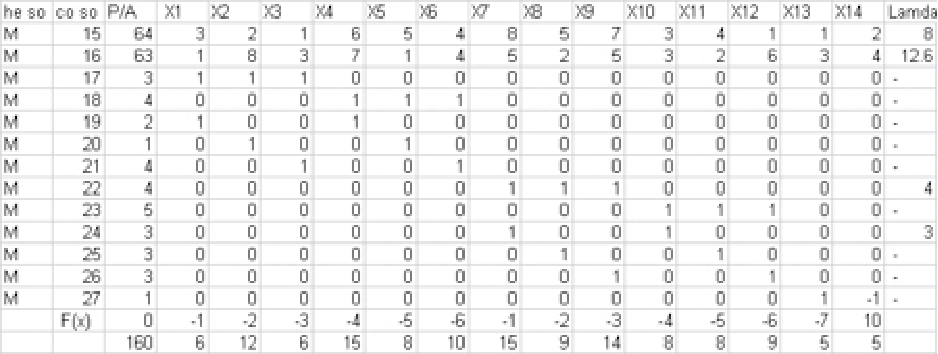
\includegraphics{lap1.pdf}
\caption{Bảng đơn hình ở bước lặp thứ 1}
\end{center}
\end{figure}
\begin{verbatim}

\end{verbatim}
\begin{figure}[!ht]
\begin{center}
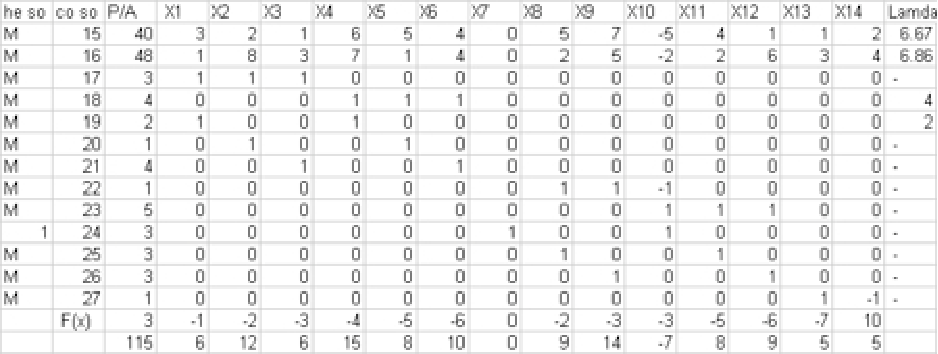
\includegraphics{lap2.pdf}
\caption{Bảng đơn hình tại bước lặp thứ 2}
\end{center}
\end{figure}
\begin{verbatim}







\end{verbatim}
\begin{figure}[!ht]
\begin{center}
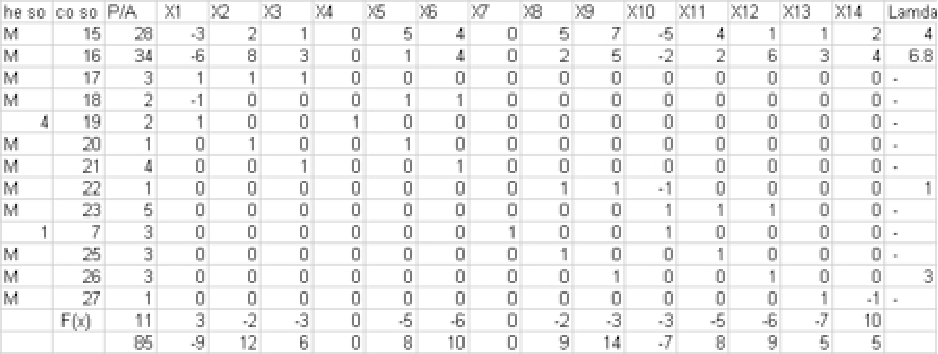
\includegraphics{lap3.pdf}
\caption{Bảng đơn hình ở bước lặp thứ 3}
\end{center}
\end{figure}

\begin{figure}[!ht]
\begin{center}
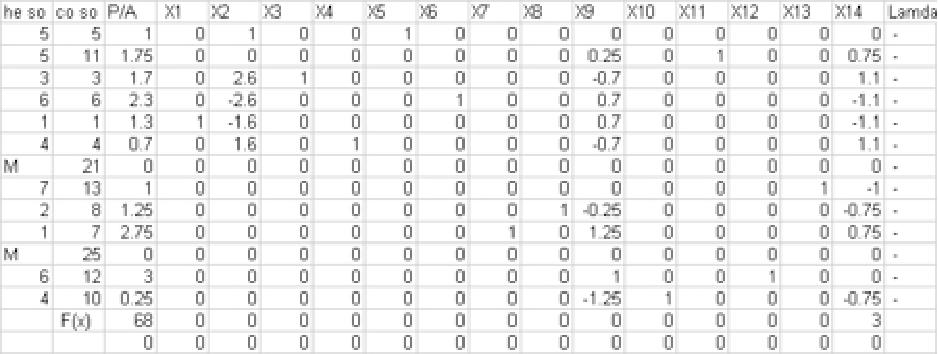
\includegraphics{lap15.pdf}
\caption{bảng đơn hình ở bước lặp thứ 15}
\end{center}
\end{figure}
\begin{verbatim}













\end{verbatim}
%+ KET THUC PHAN PHU LUC.
%+ ======================================================================================================================